\chapter[Introdução]{Introdução}

\section{Contexto}
A tecnologia tem vindo a evoluir rapidamente e, com isto, nota-se o surgimento de
diversos desafios. Um destes desafios é a falta de programadores que possuam competências 
e qualificação necessárias para solucionar os mais diversos problemas presentes nos mais
variados projetos. Este fato está relacionado com a metodologia adotada no ensino de
programação e também com a falta de motivação por parte dos estudantes \cite{7975788}.
\citeonline{inproceedings} afirmam que, uma das razões de os alunos não absorverem eficientemente
os conceitos relacionados à programação se dá pela falta de concentração e motivação dos mesmos frente
a exposição destes conteúdos na forma tradicional.

\citeonline{funcional} destaca que a aprendizagem dos conceitos e mecanismos envolvidos na construção de programas não é
trivial, uma vez que requer a utilização de raciocínio na sua forma mais abstrata. Um dos problemas mais comuns segundo os autores
são: dificuldades no entendimento de comandos, sintaxe dos comandos, dificuldades em entender os resultados da execução de um determinado 
comando pela máquina, dificuldades em dar os primeiros passos relativos ao estudo de programação entre outros.

\citeonline{ambap} diz que, em geral, os alunos têm grandes dificuldades em compreender e aplicar os conceitos relativos à programação . Uma das grandes 
dificuldades está relacionada a problemas de compreensão e aplicação de noções básicas, como por exemplo o uso de estruturas de controle e estruturas
condicionais.

Dificuldades como estas apresentadas, encorajam o desenvolvimento de soluções que auxiliem no ensino e aprendizagem de programação de forma diferente ao
atual modelo de ensino. Diversas abordagens de ensino são estudadas para facilitar o aprendizado dos alunos, algumas delas são:
gamificação, programação imperativa, programação funcional e etc. Neste trabalho, é abordado o uso da gamificação na construção de uma ferramenta
de apoio ao ensino e aprendizagem de programação desenvolvida com base nos requisitos identificados a partir da interação com ex alunos
da disciplina de Algoritmos de Programação de Computadores, ofertada pela Universidade de Brasília, campus Gama.

Segundo \citeonline{6624228}, jogos bem projetados representam bons motivadores, uma vez que passa a sensação de satisfação
e recompensa fazendo com que os jogadores persistam e fiquem engajados em realizar sua missões. Neste contexto, este poder
motivacional dos jogos, passou a ser utilizado em outros contextos que não estão relacionados diretamente aos jogos, uma prática 
conhecida atualmente como Gamificação do inglês \textit{gamification} {\itshape}.

Para \citeonline{Deterding:2011:GDE:2181037.2181040}, o termo gamificação pode ser definido como a utilização de elementos e mecânica de 
jogos em contextos não relacionados a jogos. De acordo com \citeonline{Brazil} a utilização destes elementos tornam tarefas reais em atividades
mais atrativas e lúdicas e, consequentemente, aumentam a motivação e engajamento. Há uma grande variedade de ambientes que possuem 
elementos semelhantes a características de jogos, muitos deles contendo: sistema de pontuação, feedbacks constantes e 
etc \cite{6624228}. São exemplos de ambientes com características semelhantes a de jogos: Uri, Datacamp, Edx entre outras.

A aprendizagem baseada na gamificação, preocupa-se em utilizar de mecanismos de jogos não para o entretenimento,
mas para o ensino. Os interessados no campo da gamificação trabalham para identificar o cenário e as condições 
que possam apoiar a integração de jogos aos ambientes de aprendizado. Vários cientistas e estudiosos no campo
da gamificação apontaram uma diversidade de elementos de jogos que permitem que eles sejam utilizados como
ferramentas de apoio ao aprendizado. Por exemplo: os jogos são bastante envolventes \cite{Dickey2005} e motivadores \cite{Prensky:2003:DGL:950566.950596}. Além destas características,
jogos são excelentes fontes para se adquirir experiência que são dificeis de serem fornecidas por meio de instruções tradicionais \cite{Arena2014}.

Os ambientes online gamificados de apoio ao ensino podem fornecer diversas ferramentas, entre elas: classificações, batalhas, fórums de discussões e etc.
De forma a incentivar os usuários a participarem das atividades propostas. 
Durante as competições e batalhas, os estudantes têm a possibilidade de aprender com outros jogadores e comparar suas habilidades, tornando o aprendizado mais
prazeroso \cite{LearningProgramming}. 

\pagebreak

\section{Justificativa}
De acordo com \citeonline{de2009visualg}, a abordagem de ensino tradicional de programação, que é aquela onde o professor apresenta
uma série de conceitos aos alunos e os mesmos têm a tarefa de entender como se aplicam na resolução de problemas,
para a maioria dos estudantes, se revelam muito abstratas.

Em seu trabalho de conclusão de curso pela Universidade de Brasília , campus Gama (FGA), \citeonline{calixto} apresenta uma pesquisa 
baseada nos dados referentes aos índices de aprovação, trancamento e reprovação dos alunos na disciplina de computação básica (atualmente
a disciplina recebe o nome de Algoritmos e Programação de Computadores, ofertada no campus Gama). 

Os dados utilizados por \citeonline{calixto}, são referentes a um total de 60 turmas e 3286 alunos matrículados nas disciplinas de Computação Básica entre
os anos de 2009 e 2013. Segundo o autor, dos 3286 alunos matriculados, 1659 alunos (50,48\%) foram reprovados, 262 alunos (8\%) trancaram
a disciplina e apenas 1364 alunos (41,5\%) obtiveram aprovação. O autor ainda explica que esses resultados, quando comparados à média nacional de 
aprovação de alunos em disciplinas de programação são bem preocupantes, a taxa apresentada como média nacional é de cerca de 67\% de aprovação, ou 
seja, a taxa de aprovação na FGA, é mais de 30\% menor em relação a média apresentada (67\%).

Contando com a cooperação dos funcionários da secretaria da FGA, obteve-se dados atuais referentes às aprovações, reprovações e trancamentos dos
alunos entre os períodos 2017/1 e 2019/1. Ao analisar estes dados, notou-se que do total de alunos matriculados (2225 alunos divididos em 37 turmas) no decorrer
de 5 semestres, 890 alunos (40\%) foram reprovados, 112 alunos realizaram o trancamento (5\%) e apenas 1223 alunos foram aprovados (54,96\%). Estes dados são preocupantes 
e demonstram a atual situação do aprendizado dos alunos na disciplina de Algoritmos e Programação de Computadores na FGA.

Um estudo realizado pela Universidade Federal da Paraíba (UFPB) que analisou por seis períodos 
acadêmicos os índices de reprovação na disciplina de Introdução à programação, apontou que 
em nenhum dos seis períodos analisados houvera um índice de aprovação superior a 34\%. Além disso,
os índices de reprovação e trancamento da disciplina giraram em torno dos 64\% e 6\% respectivamente \cite{SBIE6739}.

Um outro estudo, realizado na Faculdade de Educação Tecnológica do Estado do Rio de Janeiro (FAETERJ-Paracambi) por \citeonline{vieira2015dificuldades}, 
envolvendo 663 alunos da disciplina de Algoritmos 1 mostrou que, destes alunos, apenas 511 cursaram a disciplina 
até o final, ou seja, cerca de 152 alunos desistiram da disciplina. Do total restante (511), apenas 30\% foram
diretamente aprovados (cerca de 153 alunos), 40\% foram reprovados diretamente (204 alunos) e 30\% foram para o exame final (recuperação, 153).
Dos 153 alunos que foram para a recuperação, apenas 55\% foram aprovados (84 alunos), nota-se então que, dos 663 alunos que
foram matriculados na disciplina, apenas  288 alunos foram aprovados ao seu término, cerca de 43\%.

\section{Problema}
Nas seções anteriores, apresentou-se alguns estudos realizados a respeito da situação encontrada durante as análises iniciais do ensino e aprendizagem
de programação em matérias introdutórias, a partir destes panoramas, o presente trabalho visa demonstrar os resultados e passos dados na construção de uma
ferramenta gamificada para auxiliar o ensino e aprendizagem de programação.
 
\section{Objetivos}
Tendo sido apresentado o contexto e problema, o objetivo geral do presente trabalho é demonstrar o desenvolvimento e resultados
obtidos durante a construção da mesma.

Para alcançar o objetivo geral, foram definidos os seguintes objetivos específicos:
\begin{itemize}
	\item Desenvolvimento da ferramenta gamificada com base nos requisitos;
	\item Definição do método de coleta de dados a respeito da utilização da ferramenta pelos usuários;
	\item Análise dos dados a respeito da experiência de uso.
\end{itemize}

\chapter{Referencial teórico}

\section{Aprendizagem de programação}
De acordo com \citeonline{KOLIVER}, disciplinas introdutórias de programação são, em sua maioria, problemáticas e costumam apresentar
altos índices de desistência e reprovações. Um dos motivos para tal ocorrência se dá pela falta de preparo que se espera que alunos
ingressantes nestas disciplinas possuam.

Disciplina de algoritmos são normalmente oferecidas no início da grade curricular dos cursos. Isso faz com que a maioria dos alunos
cursantes sejam calouros que ainda estão acostumados com a forma ``mecanisada'' de ensino que os habituam a somente aplicar fórmulas 
sem qualquer tipo de análise mais profunda dos problemas \cite{KOLIVER}.

De acordo com \citeonline{Borges}, o modo tradicional de ensino (figura \ref{figura4}) não é suficiente para motivar os alunos a se
interessarem por disciplinas de programação. Não fica claro para a maioria dos alunos, principalmente para aqueles
não possuem nenhum tipo de conhecimento em informática, a importância de certos conteúdos.

\begin{figure}[h]
	\centering
	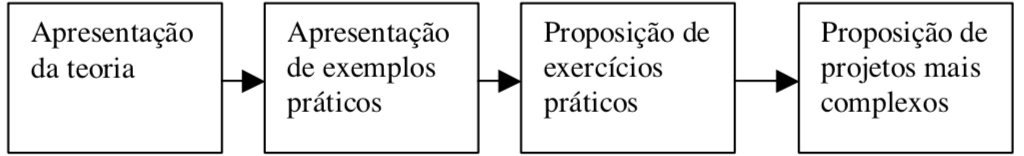
\includegraphics[keepaspectratio=true,scale=0.34]{figuras/modoTradicional.png}
	\caption{Sequência de passos típicos na apresentação de uma disciplina}
	Fonte: \cite{Borges}
	\label{figura4}
\end{figure}

Ao se apresentar uma nova liguagem de programação, é comum as aulas serem realizadas em laboratórios com
recursos computacionais. Apesar dessas aulas apresentarem um formato diferenciado em relação ao modo tradicional,
os professores não exploram a diversidade dos equipamentos disponíveis com práticas que apoiem o desenvolvimento 
de habilidades por parte dos estudantes \cite{Borges}.

\section{Gamificação}
Jogos são uma construção humana que envolvem em seu contexto fatores sociais, culturais e econômicos \cite{EaDF440}.
Como apresentado no livro ``Gamificação na Educação'' por \citeonline{da2014gamificaccao}, a interação com \textit{games}, apesar
dos custos altos dos consoles, foram ocupando cada vez mais o tempo das pessoas que notaram que os jogos poderiam ser boas fontes
de prazer e entretenimento.

O notável crescimento do mercado dos \textit{games} tem atraido diferentes olhares de estudiosos que se dedicam ao estudo de seu
uso na educação, comunicação, marketing, psicologia, computação, entre outras áreas \cite{da2014gamificaccao}.

O termo gamificação, segundo \citeonline{da2014gamificaccao}, consiste na utilização de elementos de jogos em 
atividades que por natureza de sua criação não são jogos. \citeonline{raposo2016desafio} dizem que o objetivo da gamificação, consiste em resolver
problemas práticos ou despertar interesse e engajar um público específico para a realização de uma determinada
atividade. 

Para \citeonline{chou2017actionable}, a gamificação é uma arte que é capaz de derivar elementos divertidos e envolventes encontrados em jogos e utiliza-los
em outras atividades. Para o autor, o foco deve estar centrado no ser humano e na sua motivação.

\subsection{Gamificação na Educação}
Embora o termo gamificação tenha sido apresentado pela primeira vez em 2010, a idéia de se utilizar
elementos de jogos em atividades que não são jogos, tem sido utilizado há muito tempo. Na educação
de crianças, por exemplo, as mesmas podiam ter seus esforços e trabalhos reconhecidos por meio
de estrelinhas ou outros tipos de recompensas dadas por seus educadores, como explica \citeonline{da2014gamificaccao}.

De acordo com \citeonline{da2014gamificaccao}, no Brasil existem diversas instituições públicas e privadas que apoiam o desenvolvimento e uso de ambientes
gamificados. A exemplo disto, o Ministério da Educação visa fornecer suporte para o ambiente gamificado de apoio ao ensino \textit{Geekie games} que possibilita
aos estudantes se prepararem para o Exame Nacional de Ensino Médio (ENEM). Os resultados da utilização da ferramenta, segundo \citeonline{da2014gamificaccao}, 
foram considerados positivos e o Ministério da Educação levanta a possibilidade de extender o uso da ferramenta gamificada para outros sistemas de avaliação.

Segundo \citeonline{hammer}, somente a utilização de elementos de jogos no ensino não resolve a falta de empatia no processo de aprendizagem dos alunos
uma vez que a utilização de mecanismos como por exemplo o sistema de pontuação já estão presentes no cotidiano escolar há anos. De acordo com as autoras, 
a utilização de elementos e característica de jogos devem provocar impactos tanto emocionais quanto sociais nos indivíduos para que eles tenham um aprendizado
efetivo. 

\section{Diagrama entidade-relacionamento}
Segundo \citeonline{projetobancodedados} , a abordagem mais utilizada e conhecida é a 
entidade-relacionamento (ER) onde o modelo de dados é geralmente representado graficamente através
de um diagrama entidade-relacionamento (DER). Esta abordagem foi criada em 1976 por Peter Chen e
é considerada como um padrão para a modelagem conceitual.

A abordagem entidade-relacionamento é baseada em dois principais pilares que são apresentados em seguida.

\subsection{Entidade}
De acordo com \citeonline{projetobancodedados}, uma entidade, no modelo conceitual, representa um conjunto
de objetos da realidade modelada. Seu principal objetivo é modelar de forma abstrata um banco de dados, onde
se te interesse somente nos objetos sobre os quais deseja-se manter informações. No DER, uma entidade é representada
por meio de um retângulo contendo o nome da entidade.
 
\subsection{Relacionamento}
Como apresentado por \citeonline{projetobancodedados}, o DER permite a especificar as propriedades dos objetos
que serão armazenados no banco de dados, como por exemplo o relacionamento/associação entre os objetos. No DER,
um relacionamento é representado por meio de um losango que são ligados por linhas aos retângulos que representam
as entidades que participam de um determinado relacionamento.

Na figura \ref{figura1} é apresentado um exemplo simples de um diagrama entidade-relacionamento (DER). É possível notar 
no diagrama a existência de atributos e cardinalidade, estes dois são apresentados logo em seguida.

\begin{figure}[h]
	\centering
	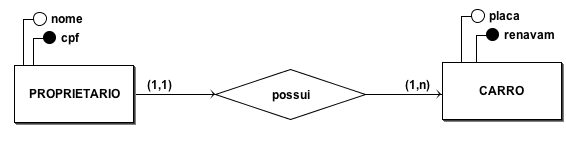
\includegraphics[keepaspectratio=true,scale=0.5]{figuras/figura1.png}
	\caption{Exemplo de DER}
	Fonte: Autor
	\label{figura1}
\end{figure}

Os atributos correspondem às características/qualidades que descrevem uma entidade, são representados por
elipses ou círculos acompanhados por seus respectivos nomes \cite{sistemadebancos}.

As cardinalidades representam a restrição do número de objetos que podem participar do relacionamento. Na notação
de Peter Chen, as cardinalidade são apresentadas próximas às ligações de relacionamento e são compostas da quantidade
mínima e máxima de objetos que podem participar do relacionamento. Tais características podem ser vistas 
na figura \ref{figura1} \cite{sistemadebancos}.

\section{Diagrama Lógico}



\chapter{Características da ferramenta}

Neste capítulo são apresentados os elementos característicos da ferramenta como: personagens, narrativa, temática entre outros 
elementos que foram pensados como forma de gamificar as atividades de aprendizagem de programação.

\section{Narrativa}

Com o objetivo de aumentar o engajamento dos estudantes/jogadores, fora desenvolvida uma história que se passa em um mundo 
onde criaturas (Orcs) invadem o vilarejo do jogador que, motivado pelo desejo de vingança e tendo sido escolhido entre uma legião 
de outros guerreiro, dá início à jornada onde o mesmo deve cumprir com desafios como: quiz, desafiar outros jogadores entre outras
atividades que dão ao jogador pontos que podem ser trocados por itens ou serem acumulados afim de obter boas posições nos \textit{rankings}.

\section{Personagens}

Ao jogador, após a realização do primeiro \textit{login} na ferramenta, são apresentados seis personagens com diferentes características, onde o jogador
deve selecionar um único personagem para iniciar a jornada de aprendizado. Ao selecionar um determinado personagem, não é permitido ao jogador/estudante 
modifica-lo no decorrer do uso da ferramenta.

Os personagens são apresentados a seguir.

\subsection{Aisha}
\begin{figure}[h]
	\centering
	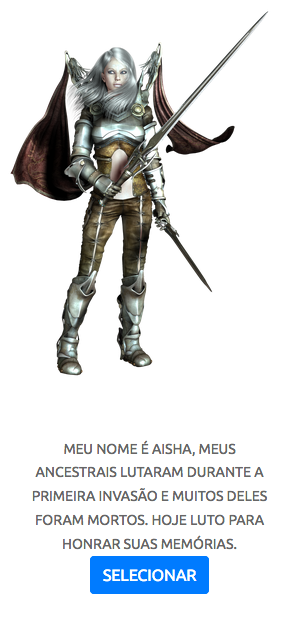
\includegraphics[keepaspectratio=true,scale=0.5]{figuras/aisha.png}
	\caption{Personagem Aisha}
	Fonte: Autor
	\label{aisha}
\end{figure}

\clearpage

\subsection{Voxter}
\begin{figure}[h]
	\centering
	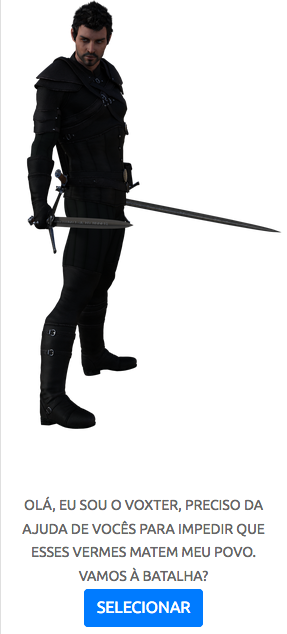
\includegraphics[keepaspectratio=true,scale=0.5]{figuras/voxter.png}
	\caption{Personagem Voxter}
	Fonte: Autor
	\label{voxter}
\end{figure}

\clearpage


\subsection{Lince}
\begin{figure}[h]
	\centering
	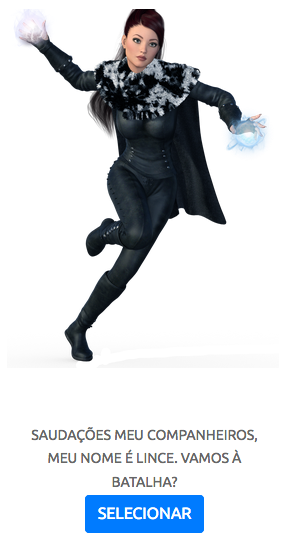
\includegraphics[keepaspectratio=true,scale=0.5]{figuras/lince.png}
	\caption{Personagem Lince}
	Fonte: Autor
	\label{lince}
\end{figure}

\clearpage

\subsection{Amazona}
\begin{figure}[h]
	\centering
	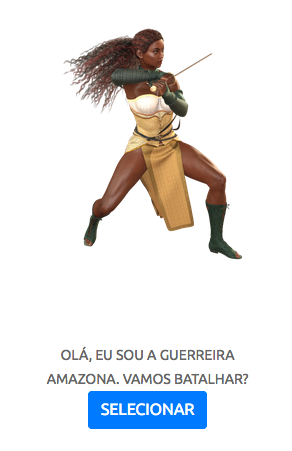
\includegraphics[keepaspectratio=true,scale=0.5]{figuras/amazona.png}
	\caption{Personagem Amazona}
	Fonte: Autor
	\label{amazona}
\end{figure}

\clearpage

\subsection{Tymer}
\begin{figure}[h]
	\centering
	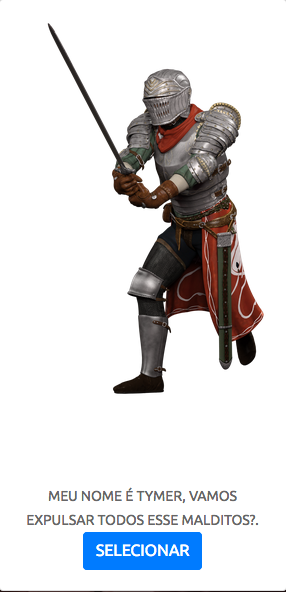
\includegraphics[keepaspectratio=true,scale=0.5]{figuras/tymer.png}
	\caption{Personagem Tymer}
	Fonte: Autor
	\label{tymer}
\end{figure}
\clearpage

\subsection{Scar}
\begin{figure}[h]
	\centering
	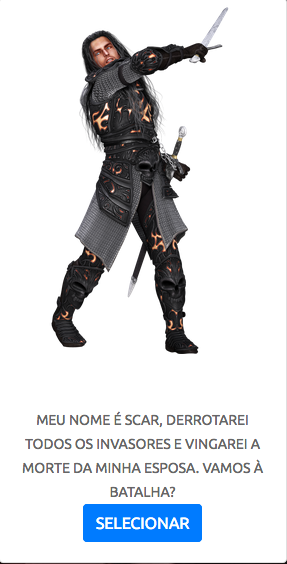
\includegraphics[keepaspectratio=true,scale=0.5]{figuras/scar.png}
	\caption{Personagem Scar}
	Fonte: Autor
	\label{scar}
\end{figure}

\chapter{Implementação da solução}

\section{Modelagem de dados}

\begin{figure}[h]
	\centering
	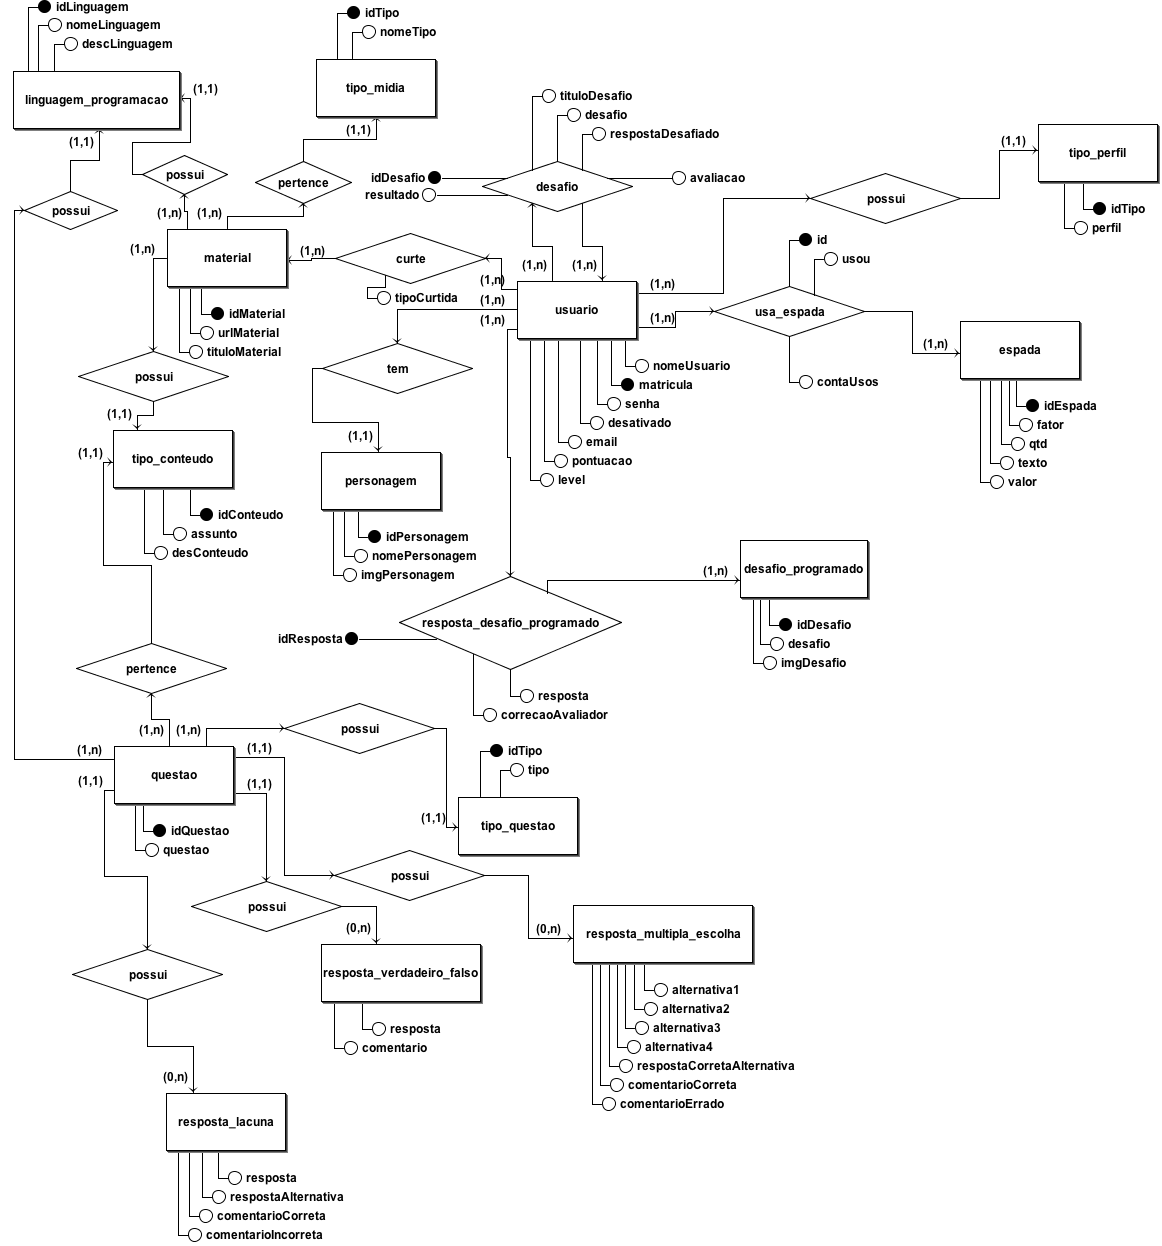
\includegraphics[keepaspectratio=true,scale=0.4]{figuras/der.png}
	\caption{DER da ferramenta}
	Fonte: Autor
	\label{figura2}
\end{figure}


\begin{figure}[h]
	\centering
	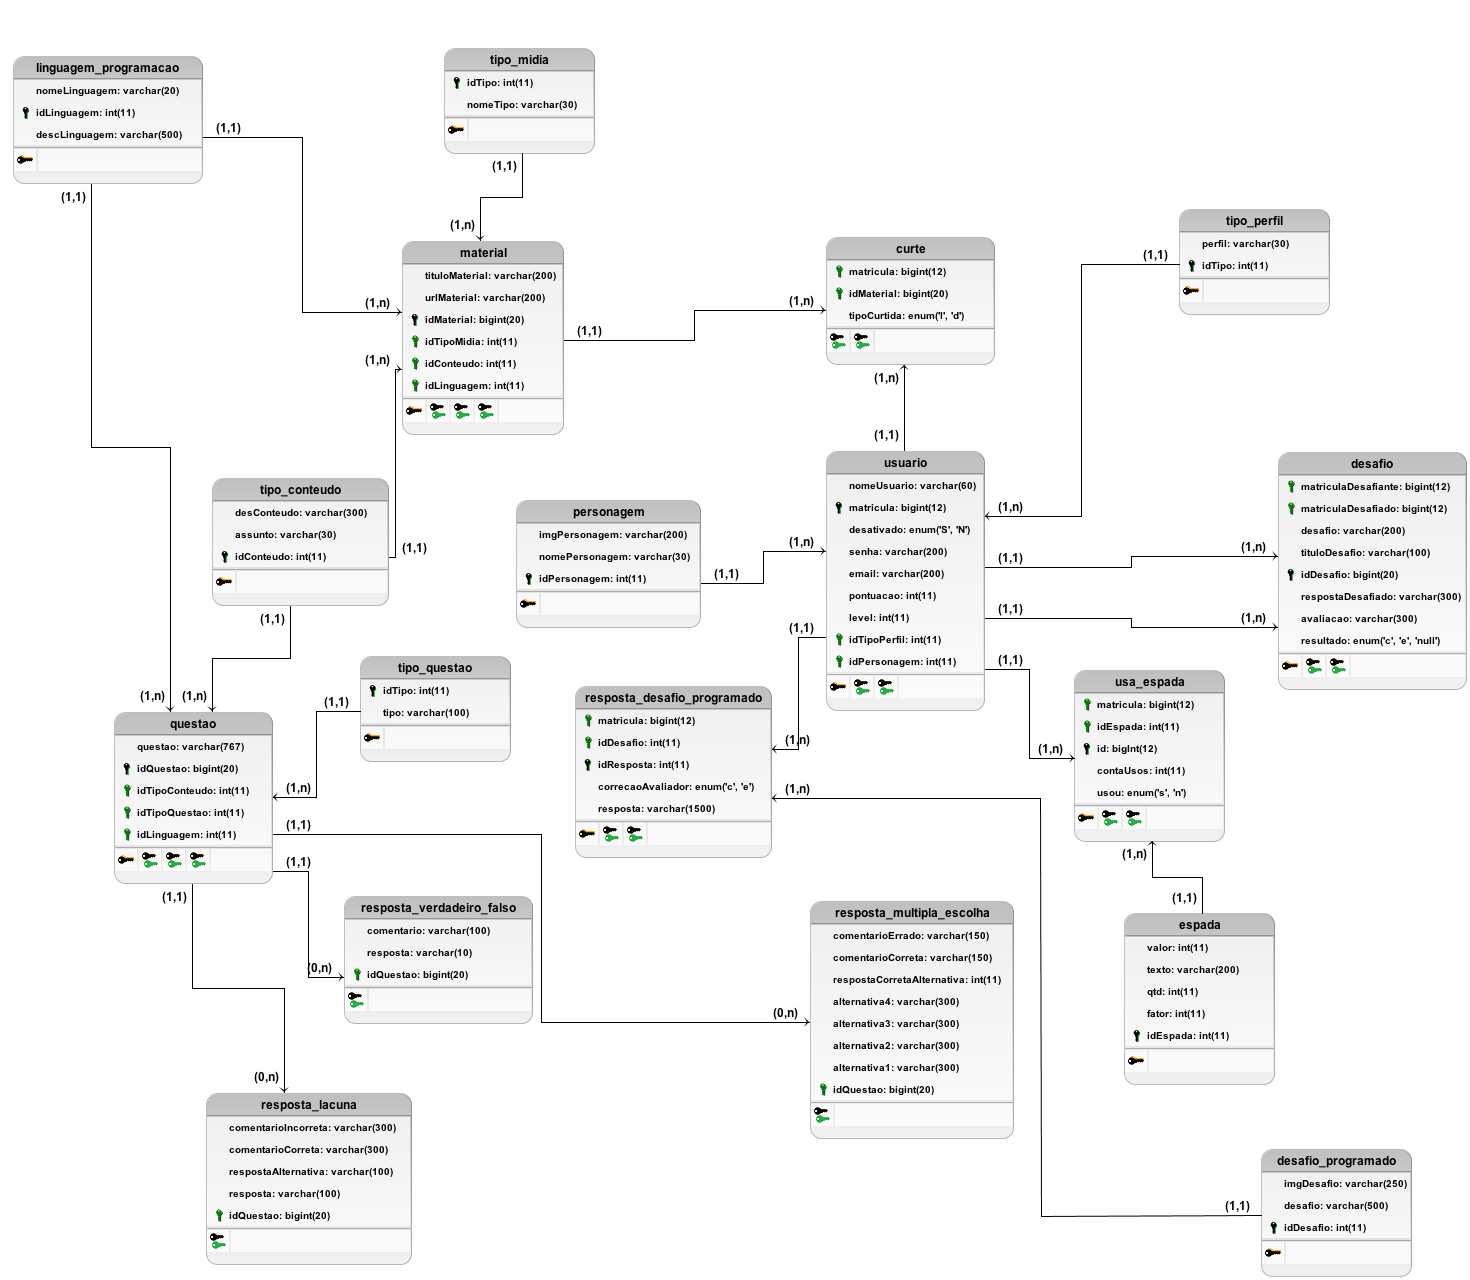
\includegraphics[keepaspectratio=true,scale=0.32]{figuras/dl.png}
	\caption{DL da ferramenta}
	Fonte: Autor
	\label{figura3}
\end{figure}





